\documentclass[twoside]{book}

% Packages required by doxygen
\usepackage{fixltx2e}
\usepackage{calc}
\usepackage{doxygen}
\usepackage[export]{adjustbox} % also loads graphicx
\usepackage{graphicx}
\usepackage[utf8]{inputenc}
\usepackage{makeidx}
\usepackage{multicol}
\usepackage{multirow}
\PassOptionsToPackage{warn}{textcomp}
\usepackage{textcomp}
\usepackage[nointegrals]{wasysym}
\usepackage[table]{xcolor}

% Font selection
\usepackage[T1]{fontenc}
\usepackage[scaled=.90]{helvet}
\usepackage{courier}
\usepackage{amssymb}
\usepackage{sectsty}
\renewcommand{\familydefault}{\sfdefault}
\allsectionsfont{%
  \fontseries{bc}\selectfont%
  \color{darkgray}%
}
\renewcommand{\DoxyLabelFont}{%
  \fontseries{bc}\selectfont%
  \color{darkgray}%
}
\newcommand{\+}{\discretionary{\mbox{\scriptsize$\hookleftarrow$}}{}{}}

% Page & text layout
\usepackage{geometry}
\geometry{%
  a4paper,%
  top=2.5cm,%
  bottom=2.5cm,%
  left=2.5cm,%
  right=2.5cm%
}
\tolerance=750
\hfuzz=15pt
\hbadness=750
\setlength{\emergencystretch}{15pt}
\setlength{\parindent}{0cm}
\setlength{\parskip}{3ex plus 2ex minus 2ex}
\makeatletter
\renewcommand{\paragraph}{%
  \@startsection{paragraph}{4}{0ex}{-1.0ex}{1.0ex}{%
    \normalfont\normalsize\bfseries\SS@parafont%
  }%
}
\renewcommand{\subparagraph}{%
  \@startsection{subparagraph}{5}{0ex}{-1.0ex}{1.0ex}{%
    \normalfont\normalsize\bfseries\SS@subparafont%
  }%
}
\makeatother

% Headers & footers
\usepackage{fancyhdr}
\pagestyle{fancyplain}
\fancyhead[LE]{\fancyplain{}{\bfseries\thepage}}
\fancyhead[CE]{\fancyplain{}{}}
\fancyhead[RE]{\fancyplain{}{\bfseries\leftmark}}
\fancyhead[LO]{\fancyplain{}{\bfseries\rightmark}}
\fancyhead[CO]{\fancyplain{}{}}
\fancyhead[RO]{\fancyplain{}{\bfseries\thepage}}
\fancyfoot[LE]{\fancyplain{}{}}
\fancyfoot[CE]{\fancyplain{}{}}
\fancyfoot[RE]{\fancyplain{}{\bfseries\scriptsize Generated by Doxygen }}
\fancyfoot[LO]{\fancyplain{}{\bfseries\scriptsize Generated by Doxygen }}
\fancyfoot[CO]{\fancyplain{}{}}
\fancyfoot[RO]{\fancyplain{}{}}
\renewcommand{\footrulewidth}{0.4pt}
\renewcommand{\chaptermark}[1]{%
  \markboth{#1}{}%
}
\renewcommand{\sectionmark}[1]{%
  \markright{\thesection\ #1}%
}

% Indices & bibliography
\usepackage{natbib}
\usepackage[titles]{tocloft}
\setcounter{tocdepth}{3}
\setcounter{secnumdepth}{5}
\makeindex

% Hyperlinks (required, but should be loaded last)
\usepackage{ifpdf}
\ifpdf
  \usepackage[pdftex,pagebackref=true]{hyperref}
\else
  \usepackage[ps2pdf,pagebackref=true]{hyperref}
\fi
\hypersetup{%
  colorlinks=true,%
  linkcolor=blue,%
  citecolor=blue,%
  unicode%
}

% Custom commands
\newcommand{\clearemptydoublepage}{%
  \newpage{\pagestyle{empty}\cleardoublepage}%
}

\usepackage{caption}
\captionsetup{labelsep=space,justification=centering,font={bf},singlelinecheck=off,skip=4pt,position=top}

%===== C O N T E N T S =====

\begin{document}

% Titlepage & ToC
\hypersetup{pageanchor=false,
             bookmarksnumbered=true,
             pdfencoding=unicode
            }
\pagenumbering{alph}
\begin{titlepage}
\vspace*{7cm}
\begin{center}%
{\Large partial\+Docu\+Test }\\
\vspace*{1cm}
{\large Generated by Doxygen 1.8.13}\\
\end{center}
\end{titlepage}
\clearemptydoublepage
\pagenumbering{roman}
\tableofcontents
\clearemptydoublepage
\pagenumbering{arabic}
\hypersetup{pageanchor=true}

%--- Begin generated contents ---
\chapter{Group 3 gitlab repo}
\label{md__r_e_a_d_m_e}
\Hypertarget{md__r_e_a_d_m_e}
Nothing to see here yet...

Something to test merge requests. 
\chapter{Hierarchical Index}
\section{Class Hierarchy}
This inheritance list is sorted roughly, but not completely, alphabetically\+:\begin{DoxyCompactList}
\item Exception\begin{DoxyCompactList}
\item \contentsline{section}{Git\+Repo.\+Url\+Exception}{\pageref{class_git_repo_1_1_url_exception}}{}
\begin{DoxyCompactList}
\item \contentsline{section}{Git\+Repo.\+No\+Url\+Specified}{\pageref{class_git_repo_1_1_no_url_specified}}{}
\item \contentsline{section}{Git\+Repo.\+Wrong\+Url\+Format}{\pageref{class_git_repo_1_1_wrong_url_format}}{}
\end{DoxyCompactList}
\end{DoxyCompactList}
\item \contentsline{section}{Git\+Repo.\+Git\+Repo}{\pageref{class_git_repo_1_1_git_repo}}{}
\end{DoxyCompactList}

\chapter{Class Index}
\section{Class List}
Here are the classes, structs, unions and interfaces with brief descriptions\+:\begin{DoxyCompactList}
\item\contentsline{section}{\hyperlink{class_git_repo_1_1_git_repo}{Git\+Repo.\+Git\+Repo} \\*Class that provides all he neccessary funcitonality associated with git repos }{\pageref{class_git_repo_1_1_git_repo}}{}
\item\contentsline{section}{\hyperlink{class_git_repo_1_1_no_url_specified}{Git\+Repo.\+No\+Url\+Specified} }{\pageref{class_git_repo_1_1_no_url_specified}}{}
\item\contentsline{section}{\hyperlink{class_git_repo_1_1_url_exception}{Git\+Repo.\+Url\+Exception} }{\pageref{class_git_repo_1_1_url_exception}}{}
\item\contentsline{section}{\hyperlink{class_git_repo_1_1_wrong_url_format}{Git\+Repo.\+Wrong\+Url\+Format} }{\pageref{class_git_repo_1_1_wrong_url_format}}{}
\end{DoxyCompactList}

\chapter{Class Documentation}
\hypertarget{class_git_repo_1_1_git_repo}{}\section{Git\+Repo.\+Git\+Repo Class Reference}
\label{class_git_repo_1_1_git_repo}\index{Git\+Repo.\+Git\+Repo@{Git\+Repo.\+Git\+Repo}}


Class that provides all he neccessary funcitonality associated with git repos.  


\subsection*{Public Member Functions}
\begin{DoxyCompactItemize}
\item 
\mbox{\Hypertarget{class_git_repo_1_1_git_repo_a345a70fa596115c9299edcbde6f05635}\label{class_git_repo_1_1_git_repo_a345a70fa596115c9299edcbde6f05635}} 
def \hyperlink{class_git_repo_1_1_git_repo_a345a70fa596115c9299edcbde6f05635}{\+\_\+\+\_\+init\+\_\+\+\_\+} (self, work\+\_\+dir=curr\+\_\+work\+\_\+dir)
\begin{DoxyCompactList}\small\item\em creates empty repository, pulled repositories will be stored here \end{DoxyCompactList}\item 
def \hyperlink{class_git_repo_1_1_git_repo_aca477c66170b04a8b16032f6fa95f056}{pull\+\_\+repo\+\_\+contents} (self, remote\+\_\+url=None, username=None, password=None)
\item 
def \hyperlink{class_git_repo_1_1_git_repo_ab0334d44a728881e4e96342e5c3bc135}{get\+\_\+commit\+\_\+data} (self)
\begin{DoxyCompactList}\small\item\em Returns the dictionary with all the neccessary information. \end{DoxyCompactList}\item 
def \hyperlink{class_git_repo_1_1_git_repo_ab1efc90018d20104eaeb8af9ef022c2a}{change\+\_\+branch} (self, branch)
\item 
\mbox{\Hypertarget{class_git_repo_1_1_git_repo_a6fafbc00a52988697f928dcd1b293d12}\label{class_git_repo_1_1_git_repo_a6fafbc00a52988697f928dcd1b293d12}} 
def \hyperlink{class_git_repo_1_1_git_repo_a6fafbc00a52988697f928dcd1b293d12}{get\+\_\+branches} (self)
\begin{DoxyCompactList}\small\item\em Returns the list of all banches in the repo. \end{DoxyCompactList}\end{DoxyCompactItemize}
\subsection*{Public Attributes}
\begin{DoxyCompactItemize}
\item 
\mbox{\Hypertarget{class_git_repo_1_1_git_repo_ae7a8a45b9f08b56c068815a376cb1f9b}\label{class_git_repo_1_1_git_repo_ae7a8a45b9f08b56c068815a376cb1f9b}} 
{\bfseries work\+\_\+dir}
\item 
\mbox{\Hypertarget{class_git_repo_1_1_git_repo_aee93693f29e2713b626b4d408c58fd10}\label{class_git_repo_1_1_git_repo_aee93693f29e2713b626b4d408c58fd10}} 
{\bfseries repo\+\_\+url}
\item 
\mbox{\Hypertarget{class_git_repo_1_1_git_repo_a8d29c7ac45aa2f793bc3644753239a90}\label{class_git_repo_1_1_git_repo_a8d29c7ac45aa2f793bc3644753239a90}} 
{\bfseries filled\+\_\+repo}
\item 
\mbox{\Hypertarget{class_git_repo_1_1_git_repo_a87d5dc3760dc2efc744ba6053599013e}\label{class_git_repo_1_1_git_repo_a87d5dc3760dc2efc744ba6053599013e}} 
{\bfseries commit\+\_\+handle}
\item 
\mbox{\Hypertarget{class_git_repo_1_1_git_repo_aa038dfda06b6459820b682b1b39c4f73}\label{class_git_repo_1_1_git_repo_aa038dfda06b6459820b682b1b39c4f73}} 
{\bfseries branches}
\end{DoxyCompactItemize}
\subsection*{Private Member Functions}
\begin{DoxyCompactItemize}
\item 
def \hyperlink{class_git_repo_1_1_git_repo_a9bb8857a25ef5927efe54dc061b37e74}{\+\_\+get\+\_\+pass} (self, locked\+\_\+url, username, password)
\item 
def \hyperlink{class_git_repo_1_1_git_repo_a831b08d2d19131c00aa6bd3eb7f6f9b7}{\+\_\+repo\+\_\+url\+\_\+test} (self, remote\+\_\+url)
\end{DoxyCompactItemize}


\subsection{Detailed Description}
Class that provides all he neccessary funcitonality associated with git repos. 



\subsection{Member Function Documentation}
\mbox{\Hypertarget{class_git_repo_1_1_git_repo_a9bb8857a25ef5927efe54dc061b37e74}\label{class_git_repo_1_1_git_repo_a9bb8857a25ef5927efe54dc061b37e74}} 
\index{Git\+Repo\+::\+Git\+Repo@{Git\+Repo\+::\+Git\+Repo}!\+\_\+get\+\_\+pass@{\+\_\+get\+\_\+pass}}
\index{\+\_\+get\+\_\+pass@{\+\_\+get\+\_\+pass}!Git\+Repo\+::\+Git\+Repo@{Git\+Repo\+::\+Git\+Repo}}
\subsubsection{\texorpdfstring{\+\_\+get\+\_\+pass()}{\_get\_pass()}}
{\footnotesize\ttfamily def Git\+Repo.\+Git\+Repo.\+\_\+get\+\_\+pass (\begin{DoxyParamCaption}\item[{}]{self,  }\item[{}]{locked\+\_\+url,  }\item[{}]{username,  }\item[{}]{password }\end{DoxyParamCaption})\hspace{0.3cm}{\ttfamily [private]}}


\begin{DoxyParams}[1]{Parameters}
\mbox{\tt in}  & {\em locked\+\_\+url} & Url of password protected repostiory \\
\hline
\mbox{\tt in}  & {\em username} & Either None or username supplied from the method call \\
\hline
\mbox{\tt in}  & {\em password} & Either None or password supplied from the method call \\
\hline
\end{DoxyParams}
\begin{DoxyReturn}{Returns}
new\+\_\+url Modified url that contains password and username reference Placeholder method that should be replaced with a nicer call 
\end{DoxyReturn}
\mbox{\Hypertarget{class_git_repo_1_1_git_repo_a831b08d2d19131c00aa6bd3eb7f6f9b7}\label{class_git_repo_1_1_git_repo_a831b08d2d19131c00aa6bd3eb7f6f9b7}} 
\index{Git\+Repo\+::\+Git\+Repo@{Git\+Repo\+::\+Git\+Repo}!\+\_\+repo\+\_\+url\+\_\+test@{\+\_\+repo\+\_\+url\+\_\+test}}
\index{\+\_\+repo\+\_\+url\+\_\+test@{\+\_\+repo\+\_\+url\+\_\+test}!Git\+Repo\+::\+Git\+Repo@{Git\+Repo\+::\+Git\+Repo}}
\subsubsection{\texorpdfstring{\+\_\+repo\+\_\+url\+\_\+test()}{\_repo\_url\_test()}}
{\footnotesize\ttfamily def Git\+Repo.\+Git\+Repo.\+\_\+repo\+\_\+url\+\_\+test (\begin{DoxyParamCaption}\item[{}]{self,  }\item[{}]{remote\+\_\+url }\end{DoxyParamCaption})\hspace{0.3cm}{\ttfamily [private]}}


\begin{DoxyParams}[1]{Parameters}
\mbox{\tt in}  & {\em remote\+\_\+url} & Reporsitory url, username and pass info will be added to this Raises an exception if there is something wrong with the url \\
\hline
\end{DoxyParams}
\mbox{\Hypertarget{class_git_repo_1_1_git_repo_ab1efc90018d20104eaeb8af9ef022c2a}\label{class_git_repo_1_1_git_repo_ab1efc90018d20104eaeb8af9ef022c2a}} 
\index{Git\+Repo\+::\+Git\+Repo@{Git\+Repo\+::\+Git\+Repo}!change\+\_\+branch@{change\+\_\+branch}}
\index{change\+\_\+branch@{change\+\_\+branch}!Git\+Repo\+::\+Git\+Repo@{Git\+Repo\+::\+Git\+Repo}}
\subsubsection{\texorpdfstring{change\+\_\+branch()}{change\_branch()}}
{\footnotesize\ttfamily def Git\+Repo.\+Git\+Repo.\+change\+\_\+branch (\begin{DoxyParamCaption}\item[{}]{self,  }\item[{}]{branch }\end{DoxyParamCaption})}


\begin{DoxyParams}[1]{Parameters}
\mbox{\tt in}  & {\em branch} & Name of the branch that you want to switch to \\
\hline
\end{DoxyParams}
\begin{DoxySeeAlso}{See also}
\hyperlink{class_git_repo_1_1_git_repo_a6fafbc00a52988697f928dcd1b293d12}{get\+\_\+branches()} method 
\end{DoxySeeAlso}
\mbox{\Hypertarget{class_git_repo_1_1_git_repo_ab0334d44a728881e4e96342e5c3bc135}\label{class_git_repo_1_1_git_repo_ab0334d44a728881e4e96342e5c3bc135}} 
\index{Git\+Repo\+::\+Git\+Repo@{Git\+Repo\+::\+Git\+Repo}!get\+\_\+commit\+\_\+data@{get\+\_\+commit\+\_\+data}}
\index{get\+\_\+commit\+\_\+data@{get\+\_\+commit\+\_\+data}!Git\+Repo\+::\+Git\+Repo@{Git\+Repo\+::\+Git\+Repo}}
\subsubsection{\texorpdfstring{get\+\_\+commit\+\_\+data()}{get\_commit\_data()}}
{\footnotesize\ttfamily def Git\+Repo.\+Git\+Repo.\+get\+\_\+commit\+\_\+data (\begin{DoxyParamCaption}\item[{}]{self }\end{DoxyParamCaption})}



Returns the dictionary with all the neccessary information. 

\begin{DoxyNote}{Note}
Merge allways returns empty list because I don\textquotesingle{}t know what else to do there 
\end{DoxyNote}
\mbox{\Hypertarget{class_git_repo_1_1_git_repo_aca477c66170b04a8b16032f6fa95f056}\label{class_git_repo_1_1_git_repo_aca477c66170b04a8b16032f6fa95f056}} 
\index{Git\+Repo\+::\+Git\+Repo@{Git\+Repo\+::\+Git\+Repo}!pull\+\_\+repo\+\_\+contents@{pull\+\_\+repo\+\_\+contents}}
\index{pull\+\_\+repo\+\_\+contents@{pull\+\_\+repo\+\_\+contents}!Git\+Repo\+::\+Git\+Repo@{Git\+Repo\+::\+Git\+Repo}}
\subsubsection{\texorpdfstring{pull\+\_\+repo\+\_\+contents()}{pull\_repo\_contents()}}
{\footnotesize\ttfamily def Git\+Repo.\+Git\+Repo.\+pull\+\_\+repo\+\_\+contents (\begin{DoxyParamCaption}\item[{}]{self,  }\item[{}]{remote\+\_\+url = {\ttfamily None},  }\item[{}]{username = {\ttfamily None},  }\item[{}]{password = {\ttfamily None} }\end{DoxyParamCaption})}


\begin{DoxyParams}[1]{Parameters}
\mbox{\tt in}  & {\em remote\+\_\+url} & Reporsitory url (by default this is None) \\
\hline
\end{DoxyParams}
\begin{DoxyReturn}{Returns}
True if repo pulled successfuly, False otherwise
\end{DoxyReturn}
The method will check if the repostitory is in valid format and create work\+Repo with contents of the user specified directory. If the repo is password protected it will request user input (password can also be specified as input arg). 

The documentation for this class was generated from the following file\+:\begin{DoxyCompactItemize}
\item 
Git\+Repo.\+py\end{DoxyCompactItemize}

\hypertarget{class_git_repo_1_1_no_url_specified}{}\section{Git\+Repo.\+No\+Url\+Specified Class Reference}
\label{class_git_repo_1_1_no_url_specified}\index{Git\+Repo.\+No\+Url\+Specified@{Git\+Repo.\+No\+Url\+Specified}}


Inheritance diagram for Git\+Repo.\+No\+Url\+Specified\+:\nopagebreak
\begin{figure}[H]
\begin{center}
\leavevmode
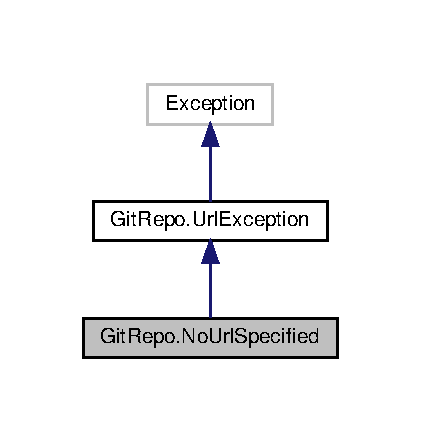
\includegraphics[width=202pt]{class_git_repo_1_1_no_url_specified__inherit__graph}
\end{center}
\end{figure}


Collaboration diagram for Git\+Repo.\+No\+Url\+Specified\+:\nopagebreak
\begin{figure}[H]
\begin{center}
\leavevmode
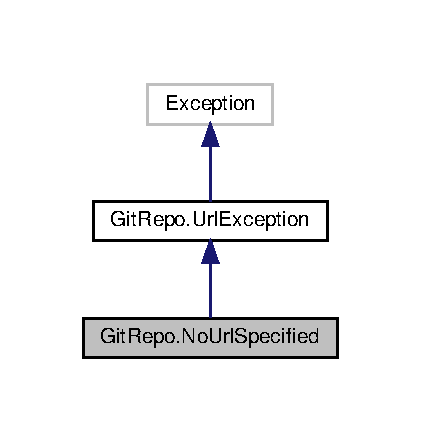
\includegraphics[width=202pt]{class_git_repo_1_1_no_url_specified__coll__graph}
\end{center}
\end{figure}


The documentation for this class was generated from the following file\+:\begin{DoxyCompactItemize}
\item 
Git\+Repo.\+py\end{DoxyCompactItemize}

\hypertarget{class_git_repo_1_1_url_exception}{}\section{Git\+Repo.\+Url\+Exception Class Reference}
\label{class_git_repo_1_1_url_exception}\index{Git\+Repo.\+Url\+Exception@{Git\+Repo.\+Url\+Exception}}


Inheritance diagram for Git\+Repo.\+Url\+Exception\+:\nopagebreak
\begin{figure}[H]
\begin{center}
\leavevmode
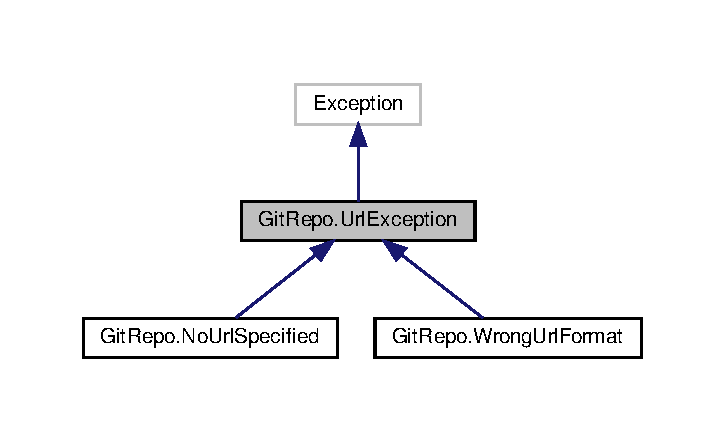
\includegraphics[width=348pt]{class_git_repo_1_1_url_exception__inherit__graph}
\end{center}
\end{figure}


Collaboration diagram for Git\+Repo.\+Url\+Exception\+:\nopagebreak
\begin{figure}[H]
\begin{center}
\leavevmode
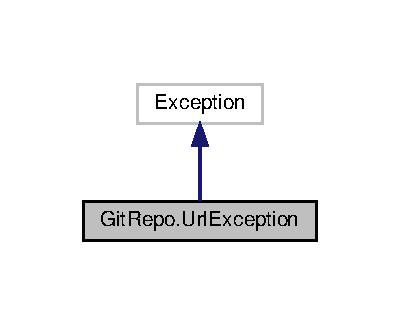
\includegraphics[width=192pt]{class_git_repo_1_1_url_exception__coll__graph}
\end{center}
\end{figure}


The documentation for this class was generated from the following file\+:\begin{DoxyCompactItemize}
\item 
Git\+Repo.\+py\end{DoxyCompactItemize}

\hypertarget{class_git_repo_1_1_wrong_url_format}{}\section{Git\+Repo.\+Wrong\+Url\+Format Class Reference}
\label{class_git_repo_1_1_wrong_url_format}\index{Git\+Repo.\+Wrong\+Url\+Format@{Git\+Repo.\+Wrong\+Url\+Format}}


Inheritance diagram for Git\+Repo.\+Wrong\+Url\+Format\+:\nopagebreak
\begin{figure}[H]
\begin{center}
\leavevmode
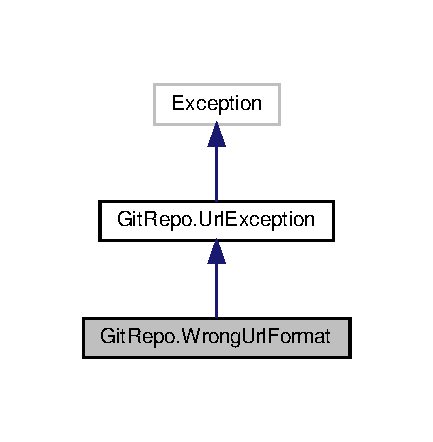
\includegraphics[width=208pt]{class_git_repo_1_1_wrong_url_format__inherit__graph}
\end{center}
\end{figure}


Collaboration diagram for Git\+Repo.\+Wrong\+Url\+Format\+:\nopagebreak
\begin{figure}[H]
\begin{center}
\leavevmode
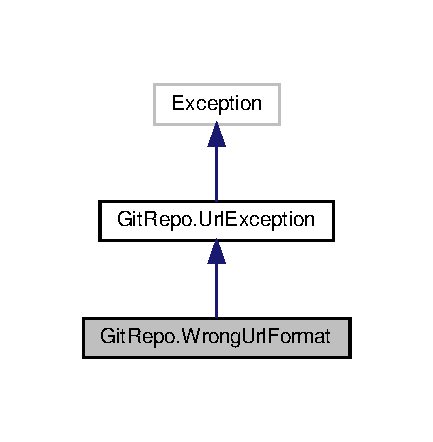
\includegraphics[width=208pt]{class_git_repo_1_1_wrong_url_format__coll__graph}
\end{center}
\end{figure}


The documentation for this class was generated from the following file\+:\begin{DoxyCompactItemize}
\item 
Git\+Repo.\+py\end{DoxyCompactItemize}

%--- End generated contents ---

% Index
\backmatter
\newpage
\phantomsection
\clearemptydoublepage
\addcontentsline{toc}{chapter}{Index}
\printindex

\end{document}
